\documentclass[24pt,t,table, aspectratio=169]{beamer}

\usetheme[progressbar=frametitle]{metropolis}
\usepackage{appendixnumberbeamer}

\usepackage{booktabs}
\usepackage[scale=2]{ccicons}
\newcommand{\themename}{\textbf{\textsc{metropolis}}\xspace}

\setbeamercolor{background canvas}{bg=white}
\usepackage{framed}
\usepackage{mdframed}
\usepackage{siunitx}
\usepackage{hyperref}
\usetikzlibrary{decorations.pathmorphing}


\newcommand{\atom}[3]{%
  \begin{scope}[shift={(#1,#2)}]
    % Proton (blue dot at center)
    \fill[blue] (0,0) circle (0.1) node[below left=2pt] {$p^+$};

    % Orbit path
    \draw[dashed,gray] (0,0) circle (0.6);

    % Electron (red dot on orbit)
    \fill[red] ({.6*cos(#3)},{.6*sin(#3)}) circle (0.1)
      node[above right=2pt] {$e^-$};
  \end{scope}%
}

\begin{document}

\begin{frame}[c, noframenumbering, plain]
  %\maketitle
  
  \large
  \begin{center}
  \begin{mdframed}[linecolor=orange, backgroundcolor=orange!20]
  \Large
  \centering
  \textbf{A Hybridized Discontinuous Galerkin Solver for Inductively Coupled Plasma}
  
  \small
  
  Nicolas Corthouts
  \end{mdframed}
  %\vspace{0.2cm}
  %\textcolor{orange}{\hrule}
  \end{center}
  \begin{center}
  \begin{tikzpicture}
  \draw (0,0) node{\includegraphics[width=.9\linewidth]{./cover_cropped.png}};
  \draw (0,-2.05) node{\reflectbox{\includegraphics[width = .9\linewidth, angle=180, origin=c]{./cover_cropped.png}}};
  \end{tikzpicture}
  \end{center}
  
%  \begin{minipage}[c]{.49\linewidth}
%  \small
%  \begin{tabular}{ll}
%  \textbf{Author} & Nicolas Corthouts\\ 
%  \textbf{Promoters} & Koen Hillewaert\\
%   & Thierry Magin
%  \end{tabular}
%  \end{minipage}
%  \begin{minipage}[c]{.49\linewidth}
%  \begin{tabular}{ll}
%  \textbf{Jury} & Christophe Geuzaine\\
%   & Peter Schütz \\
%   & Trevor Lafleur
%  \end{tabular}
%  \end{minipage}
%
%  \vspace{0.3cm}
  \includegraphics[height =1 cm]{2560px-University_of_Liège_logo.png}\hfill
\includegraphics[height=1 cm]{FRS-FNRS_ros_vert_transp.png}\hfill
\includegraphics[height =1 cm]{vki_logo_blue_rectangular.jpg}
  \vfill
\end{frame}

\section{Introduction}

\begin{frame}{Etats de la matière: eau à pression atmosphérique}

\begin{center}
\begin{tabular}{ccc}
\textbf{Solide} & \textbf{Liquide} & \textbf{Gaz}\\
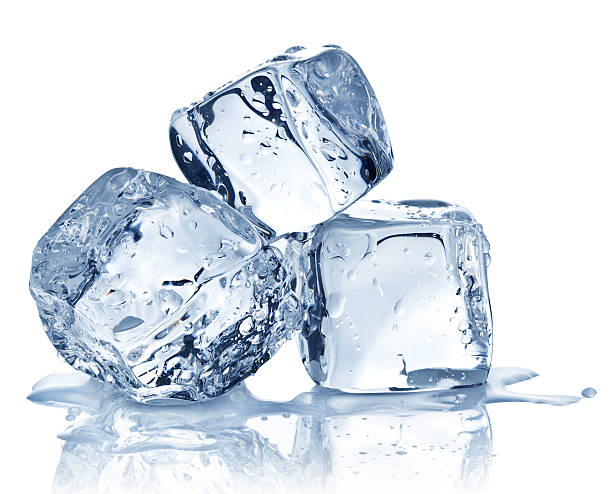
\includegraphics[height=.17\linewidth]{ice_cubes.jpg} & 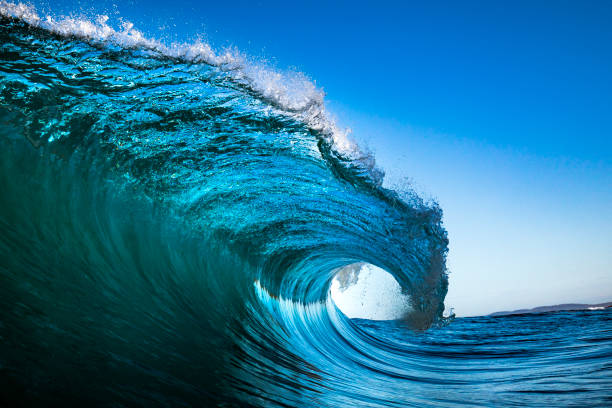
\includegraphics[height=.17\linewidth]{eau_liquide.jpg} & 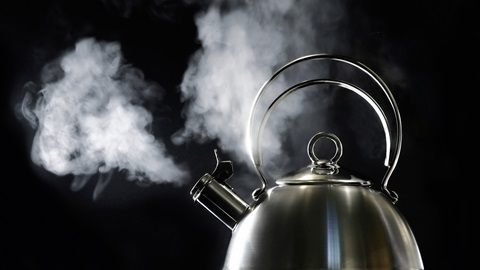
\includegraphics[height=.17\linewidth]{bouilloire.jpg}\\
\onslide<2->{
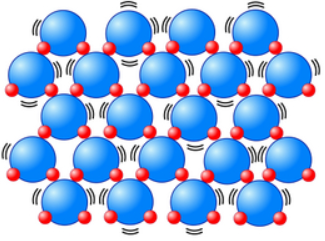
\includegraphics[height=.17\linewidth]{eau_solide.png} & 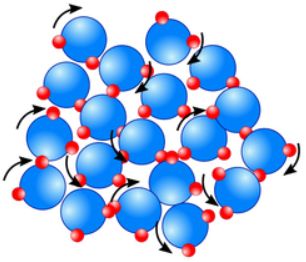
\includegraphics[height=.17\linewidth]{eau_liquide.png} & 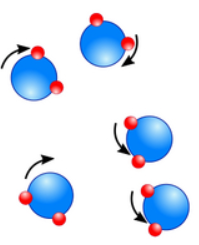
\includegraphics[height=.17\linewidth]{eau_gaz.png}\footnote{\tiny\url{https://www.assistancescolaire.com/eleve/3e/physique-chimie/reviser-une-notion/les-\%20etatsde-la-matiere-et-les-changements-d-etat-3_pc_01/print?print=1&printSheet=1}}\\
}
%\onslide<3->{
%$T \leq \SI{0}{\celsius}$ & $T \geq \SI{0}{\celsius}$ & $T \geq \SI{100}{\celsius}$
%}
\end{tabular}
\end{center}

\end{frame}

\begin{frame}{Translation, rotation et vibration}

\begin{framed}
\centering
\textbf{Que se passe-t-il si on chauffe encore plus notre eau?}
%A plasma is a quasi-neutral gas of charged and neutral particles which exhibits collective behaviour.
\end{framed}


\begin{center}
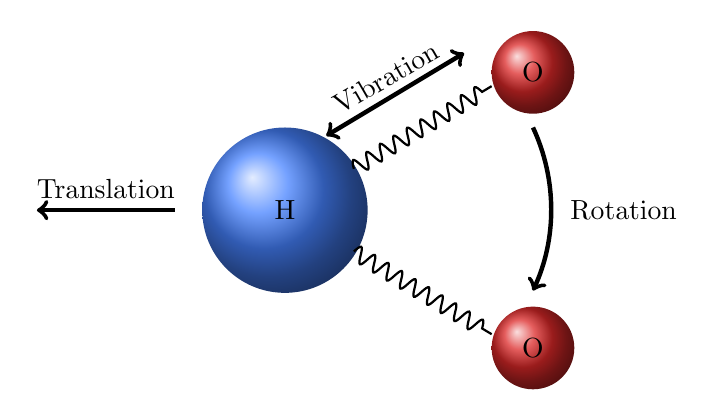
\begin{tikzpicture}[scale=3.5, spring/.style={decorate,decoration={coil,aspect=0,segment length=2mm,amplitude=1mm}}]

  % Oxygen atom color (blue)
  \definecolor{OxyBlue}{RGB}{70,130,255} % light-medium blue
  % Hydrogen atom color (red)
  \definecolor{HydRed}{RGB}{220,40,40}   % bright red

  % Oxygen atom
  \shade[ball color=OxyBlue] (0,0) circle (0.3);

  % Hydrogen atoms (approx 104° apart)
  \shade[ball color=HydRed] (0.9,0.5) circle (0.15);
  \shade[ball color=HydRed] (0.9,-0.5) circle (0.15);
  
  \node at (0,0) {H};
  \node at (0.9,0.5) {O};
  \node at (0.9,-0.5) {O};
  
  \draw[spring,thick] (0.25,0.15) -- (0.75,0.45);
  \draw[spring,thick] (0.25,-0.15) -- (0.75,-0.45);
  
  \onslide<2,5->{
  \draw[->, ultra thick] (-0.4,0) -- (-0.65,0) node[above]{Translation} -- (-0.9,0);
  }
  
  \onslide<3,5->{
  \draw[->,thick, ultra thick] (0.9,0.3) arc[start angle=25,end angle=-25,radius=.7];
  \node at (1., 0) [right]{Rotation};
  %\draw[bend right, ->, ultra thick] (0.9,-0.5) -- (0.9,0.5);
  }
  
  \onslide<4,5->{
  \draw[<->,thick, ultra thick] (0.15,0.27) -- (0.65,0.57);
  \node at (0.4, .42) [above, rotate=30] {Vibration};
  %\draw[bend right, ->, ultra thick] (0.9,-0.5) -- (0.9,0.5);
  }

  % Optional arrows to mimic rotation (as in your image)
  %\draw[->,thick] (0.35,0.55) arc[start angle=100,end angle=20,radius=0.6];
  %\draw[->,thick] (0.35,-0.55) arc[start angle=-100,end angle=-20,radius=0.6];

\end{tikzpicture}
\end{center}

%Les molécules vibrent, tournent et se déplacent de plus en plus vite. Les electrons sont excités jusqu'à ce que certains se détachent et se meuvent librement.
\end{frame}

\begin{frame}{Excitation et ionization}

\begin{center}
\begin{tikzpicture}[scale=3.5, spring/.style={decorate,decoration={coil,aspect=0,segment length=2mm,amplitude=1mm}}]

  % Oxygen atom color (blue)
  \definecolor{OxyBlue}{RGB}{70,130,255} % light-medium blue
  % Hydrogen atom color (red)
  \definecolor{HydRed}{RGB}{220,40,40}   % bright red

  % Oxygen atom
  \shade[ball color=OxyBlue] (0,0) circle (0.3);
  
  \node at (0,0) {H};
 
  \onslide<2->
  {
  	\def\dist{1.5}
  	\fill[blue] (\dist,0) circle (0.03) node[below left=2pt] {$p^+$};

  	% Orbit path (optional, dashed)
  	\draw[dashed,gray] (\dist,0) circle (.5);

	\draw[->, ultra thick] (.4, 0) -- (.9,0);

  	% Electron (red dot on orbit)
  	\def\ang{40} % position angle
  }
  
  \onslide<2>{
  	\fill[red] ({\dist+.5*cos(\ang)},{.5*sin(\ang)}) circle (0.03) 
  	node[below left] {$e^-$};
  }
  
  \onslide<3->
  {
  	\fill[red!50] ({\dist+.5*cos(\ang)},{.5*sin(\ang)}) circle (0.03) 
  	node[below left] {$e^-$};
  }  
  
  \onslide<3>
  {
  	\draw[dashed,gray] (\dist,0) circle (.7);
  	\fill[red] ({\dist+.7*cos(\ang)},{.7*sin(\ang)}) circle (0.03) 
  	node[above right] {$e^-$};
  	\draw[->, ultra thick, red] ({\dist+.55*cos(\ang)},{.55*sin(\ang)}) -- ({\dist+.65*cos(\ang)},{.65*sin(\ang)});
  }
  
  
  \onslide<4>
  {
  	%\draw[dashed,gray] (\dist,0) circle (.9);
  	\fill[red] ({\dist+.9*cos(\ang)},{.9*sin(\ang)}) circle (0.03) 
  	node[above right] {$e^-$};
  	\draw[->, ultra thick, red] ({\dist+.9*cos(\ang)+0.1},{.9*sin(\ang)}) -- ({\dist+.9*cos(\ang)+0.1+0.5},{.9*sin(\ang)});
  }

\end{tikzpicture}

\only<3>
{
	\begin{framed}
	\centering
	Si l'énergie reçue le permet, l'électron est dans un état \textcolor{red}{\textbf{excité}}. Il reviendra à son état initial en émettant de la lumière: c'est la \textbf{\textcolor{red}{radiation}}.
	\end{framed}
}

\only<4>
{
	\begin{framed}
	\centering
	Si l'énergie reçue est trop grande, l'électron est arraché: il devient \textcolor{red}{\textbf{libre}}.
	\end{framed}
}

\end{center}

\end{frame}

\end{document}